%%%---PREAMBLE---%%%%%%%%%%%%%%%%%%%%%%%%%%%%
\documentclass[twoside,12pt,final]{ucthesis-CA2012}

% fix for pandoc 1.14
\providecommand{\tightlist}{%
  \setlength{\itemsep}{0pt}\setlength{\parskip}{0pt}}

%--- Packages ---------------------------------------------------------
\usepackage[lofdepth,lotdepth,caption=false]{subfig}
\usepackage{fancyhdr}
\usepackage{amsmath, amssymb, graphicx}
\usepackage{xspace}
\usepackage{braket}
\usepackage{color}
\usepackage{setspace}
\usepackage{fancyvrb}
\usepackage{array}
\usepackage{ifxetex,ifluatex}
\usepackage{etoolbox}
\usepackage{booktabs}
\usepackage{longtable}

% suppress bottom page numbers on first page of each chapter
% because they overlap with text
\patchcmd{\chapter}{plain}{empty}{}{}

%---New Definitions and Commands------------------------------------------------------

\newtheorem{theorem}{Jibberish}

\bibliography{references}

\hyphenation{mar-gin-al-ia}

% from uw_template.tex

% commands and environments needed by pandoc snippets
% extracted from the output of `pandoc -s`
%% Make R markdown code chunks work

\ifxetex
  \usepackage{fontspec,xltxtra,xunicode}
  \defaultfontfeatures{Mapping=tex-text,Scale=MatchLowercase}
\else
  \ifluatex
    \usepackage{fontspec}
    \defaultfontfeatures{Mapping=tex-text,Scale=MatchLowercase}
  \else
    \usepackage[utf8]{inputenc}
  \fi
\fi
\DefineShortVerb[commandchars=\\\{\}]{\|}
\DefineVerbatimEnvironment{Highlighting}{Verbatim}{commandchars=\\\{\}}
% Add ',fontsize=\small' for more characters per line
\newenvironment{Shaded}{}{}
\newcommand{\KeywordTok}[1]{\textcolor[rgb]{0.00,0.44,0.13}{\textbf{{#1}}}}
\newcommand{\DataTypeTok}[1]{\textcolor[rgb]{0.56,0.13,0.00}{{#1}}}
\newcommand{\DecValTok}[1]{\textcolor[rgb]{0.25,0.63,0.44}{{#1}}}
\newcommand{\BaseNTok}[1]{\textcolor[rgb]{0.25,0.63,0.44}{{#1}}}
\newcommand{\FloatTok}[1]{\textcolor[rgb]{0.25,0.63,0.44}{{#1}}}
\newcommand{\CharTok}[1]{\textcolor[rgb]{0.25,0.44,0.63}{{#1}}}
\newcommand{\StringTok}[1]{\textcolor[rgb]{0.25,0.44,0.63}{{#1}}}
\newcommand{\CommentTok}[1]{\textcolor[rgb]{0.38,0.63,0.69}{\textit{{#1}}}}
\newcommand{\OtherTok}[1]{\textcolor[rgb]{0.00,0.44,0.13}{{#1}}}
\newcommand{\AlertTok}[1]{\textcolor[rgb]{1.00,0.00,0.00}{\textbf{{#1}}}}
\newcommand{\FunctionTok}[1]{\textcolor[rgb]{0.02,0.16,0.49}{{#1}}}
\newcommand{\RegionMarkerTok}[1]{{#1}}
\newcommand{\ErrorTok}[1]{\textcolor[rgb]{1.00,0.00,0.00}{\textbf{{#1}}}}
\newcommand{\NormalTok}[1]{{#1}}
\newcommand{\OperatorTok}[1]{\textcolor[rgb]{0.00,0.44,0.13}{\textbf{{#1}}}}
\newcommand{\BuiltInTok}[1]{\textcolor[rgb]{0.00,0.44,0.13}{\textbf{{#1}}}}
\newcommand{\ControlFlowTok}[1]{\textcolor[rgb]{0.00,0.44,0.13}{\textbf{{#1}}}}

\ifxetex
  \usepackage[setpagesize=false, % page size defined by xetex
              unicode=false, % unicode breaks when used with xetex
              xetex,
              colorlinks=true,
              linkcolor=blue]{hyperref}
\else
  \usepackage[unicode=true,
              colorlinks=true,
              linkcolor=blue]{hyperref}
\fi
\hypersetup{breaklinks=true, pdfborder={0 0 0}}
\setlength{\parindent}{0pt}
\setlength{\parskip}{6pt plus 2pt minus 1pt}
\setlength{\emergencystretch}{3em}  % prevent overfull lines
\setcounter{secnumdepth}{0}

%---Set Margins ------------------------------------------------------
\setlength\oddsidemargin{0.25 in} \setlength\evensidemargin{0.25 in} \setlength\textwidth{6.25 in} \setlength\textheight{8.50 in}
\setlength\footskip{0.25 in} \setlength\topmargin{0 in} \setlength\headheight{0.25 in} \setlength\headsep{0.25 in}

%%%---DOCUMENT---%%%%%%%%%%%%%%%%%%%%%%%%%%%%
\begin{document}

%=== Preliminary Pages ============================================
\begin{ucfrontmatter}

  %%%%%%%%%%%%%%%%%%%%%%%%%%%
  % TITLE PAGE INFORMATION %
  %%%%%%%%%%%%%%%%%%%%%%%%%%%

  \title{Linking watersheds with genomics: Population genetics of the Foothill
yellow-legged Frog (\emph{Rana boylii})}

  \author{Ryan A Peek}

  \report{Dissertation} 
  \degree{Doctor of Philosophy} 
  \degreemonth{August} \degreeyear{2018}
  %\defensemonth{August} % should be one of the following: March,
  %\defenseyear{2018}
  \chair{Michael R. Miller}  % this is your advisor
  \othermemberA{Peter B. Moyle} % This is a member of your committee
  \othermemberB{Mark W. Schwartz} % This is a member of your committee
  \othermemberC{} % This is a member of your committee (if your department requires 4 members)
  \numberofmembers{3} % should match the number of entries above (chair + othermembers)

  \field{Ecology}
  \campus{Davis}
	\maketitle
	\approvalpage
	\copyrightpage

  %%%%%%%%%%%%%%%%%%%%%%%%%%%
  % DEDICATION PAGE INFORMATION %
  %%%%%%%%%%%%%%%%%%%%%%%%%%%
    \begin{dedication}

      \vspace*{25ex}
      \begin{center}
      \begin{Large}

        To Hobbes

      \end{Large}
      \end{center}
  \end{dedication}
  \begin{acknowledgements}
    Thanks everyone!
  \end{acknowledgements}
  %%%%%%
  % CV %
  %%%%%%
  \begin{vitae}
    \addcontentsline{toc}{chapter}{Curriculum Vitae}
    \begin{vitaesection}{Education}
    \vspace{-0.1cm}
    \item [2018]	Ph.D. in Environmental Science and Management (Expected), University of California, Santa Barbara.
    \item [2010]	MESM in in Environmental Science and Management, University of California, Santa Barbara.
    \item [2007]	B.S. in Ecosystem Science and Policy and Biology, University of Miami
    \end{vitaesection}
    \textbf{Publications}

    Anderson, S.C., Cooper, A.B., Jensen, O.P., Minto, C., Thorson, J.T., Walsh, J.C., Afflerbach, J., Dickey‐Collas, M., Kleisner, K.M., Longo, C., Osio, G.C., Ovando, D., Mosqueira, I., Rosenberg, A.A., Selig, E.R., n.d. Improving estimates of population status and trend with superensemble models. Fish and Fisheries 18, 732–741. https://doi.org/10.1111/faf.12200

 Burgess, M.G., McDermott, G.R., Owashi, B., Reeves, L.E.P., Clavelle, T., Ovando, D., Wallace, B.P., Lewison, R.L., Gaines, S.D., Costello, C., 2018. Protecting marine mammals, turtles, and birds by rebuilding global fisheries. Science 359, 1255–1258. https://doi.org/10.1126/science.aao4248

Costello, C., Ovando, D., Clavelle, T., Strauss, C.K., Hilborn, R., Melnychuk, M.C., Branch, T.A., Gaines, S.D., Szuwalski, C.S., Cabral, R.B., Rader, D.N., Leland, A., 2016. Global fishery prospects under contrasting management regimes. PNAS 113, 5125–5129. https://doi.org/10.1073/pnas.1520420113

Costello, C., Ovando, D., Hilborn, R., Gaines, S.D., Deschenes, O., Lester, S.E., 2012. Status and Solutions for the World’s Unassessed Fisheries. Science 338, 517–520. https://doi.org/10.1126/science.1223389

Dowling, N., Wilson, J., Rudd, M., Babcock, E., Caillaux, M., Cope, J., Dougherty, D., Fujita, R., Gedamke, T., Gleason, M., Guttierrez, M., Hordyk, A., Maina, G., Mous, P., Ovando, D., Parma, A., Prince, J., Revenga, C., Rude, J., Szuwalski, C., Valencia, S., Victor, S., 2016. FishPath: A Decision Support System for Assessing and Managing Data- and Capacity- Limited Fisheries, in: Quinn II, T., Armstrong, J., Baker, M., Heifetz, J., Witherell, D. (Eds.), Assessing and Managing Data-Limited Fish Stocks. Alaska Sea Grant, University of Alaska Fairbansk.

Fogarty, M.J., Rosenberg, A.A., Cooper, A.B., Dickey-Collas, M., Fulton, E.A., Gutiérrez, N.L., Hyde, K.J.W., Kleisner, K.M., Kristiansen, T., Longo, C., Minte-Vera, C.V., Minto, C., Mosqueira, I., Osio, G.C., Ovando, D., Selig, E.R., Thorson, J.T., Ye, Y., 2016. Fishery production potential of large marine ecosystems: A prototype analysis. Environmental Development, SI:Ecosystem-based LME Mgt 17, Supplement 1, 211–219. https://doi.org/10.1016/j.envdev.2016.02.001

Hammerschlag, N., Ovando, D., Serafy, J.E., 2010. Seasonal diet and feeding habits of juvenile fishes foraging along a subtropical marine ecotone. Aquatic Biology 9, 279–290.
Hilborn, R., Ovando, D., 2014. Reflections on the success of traditional fisheries management. ICES J. Mar. Sci. 71, 1040–1046. https://doi.org/10.1093/icesjms/fsu034

Ovando, D., Dougherty, D., Wilson, J.R., 2016a. Market and design solutions to the short-term economic impacts of marine reserves. Fish Fish n/a-n/a. https://doi.org/10.1111/faf.12153

Ovando, D., Poon, S., Costello, C., 2016b. Opportunities and precautions for integrating cooperation and individual transferable quotas with territorial use rights in fisheries. Bulletin of Marine Science.

Ovando, D., Deacon, R.T., Lester, S.E., Costello, C., Van Leuvan, T., McIlwain, K., Strauss, K.C., Arbuckle, M., Fujita, R., Gelcich, S., Uchida, H., 2013. Conservation incentives and collective choices in cooperative fisheries. Marine Policy 37, 132–140. https://doi.org/10.1016/j.marpol.2012.03.012
Rahimi, S., Gaines, S.D., Gelcich, S., Deacon, R., Ovando, D., 2016. Factors driving the implementation of fishery reforms. Marine Policy 71, 222–228. https://doi.org/10.1016/j.marpol.2016.06.005

Rosenberg, A.A., Fogarty, M.J., Cooper, A.B., Dickey-Collas, M., Fulton, E.A., Gutiérrez, N.L., Hyde, K.J.W., Kleisner, K.M., Kristiansen, T., Longo, C., Minte-Vera, C., Minto, C., Mosqueira, I., Chato Osio, G., Ovando, D., Selig, E.R., Thorson, J.T., Ye, Y., 2014. Developing new approaches to global stock status assessment and fishery production potential of the seas, FAO Fisheries and Aquaculture Circular. Food and Agriculture Organization of the United Nations.

Rosenberg, A.A., Kleisner, K.M., Afflerbach, J., Anderson, S.C., Dickey-Collas, M., Cooper, A.B., Fogarty, M.J., Fulton, E.A., Gutiérrez, N.L., Hyde, K.J.W., Jardim, E., Jensen, O.P., Kristiansen, T., Longo, C., Minte-Vera, C.V., Minto, C., Mosqueira, I., Osio, G.C., Ovando, D., Selig, E.R., Thorson, J.T., Walsh, J.C., Ye, Y., 2017. Applying a New Ensemble Approach to Estimating Stock Status of Marine Fisheries around the World. CONSERVATION LETTERS n/a-n/a. https://doi.org/10.1111/conl.12363

Szuwalski, C.S., Castrejon, M., Ovando, D., Chasco, B., 2016. An integrated stock assessment for red spiny lobster (Panulirus penicillatus) from the Galapagos Marine Reserve. Fisheries Research 177, 82–94. https://doi.org/10.1016/j.fishres.2016.01.002


  \end{vitae}
	%%%%%%%%%%%%%%%%%%%%%%%%%%%
  % ABSTRACT %
  %%%%%%%%%%%%%%%%%%%%%%%%%%%
  \begin{abstract}
    \addcontentsline{toc}{chapter}{Abstract}
    %todo: max 350 words

    The data say `meh'

    %\abstractsignature
  \end{abstract}
	\tableofcontents
\end{ucfrontmatter}
\begin{ucmainmatter}

\hypertarget{introduction}{%
\chapter*{Introduction}\label{introduction}}
\addcontentsline{toc}{chapter}{Introduction}

Welcome to the \emph{R Markdown} thesis template. This template is based
on (and in many places copied directly from) the UW LaTeX template, but
hopefully it will provide a nicer interface for those that have never
used TeX or LaTeX before. Using \emph{R Markdown} will also allow you to
easily keep track of your analyses in \textbf{R} chunks of code, with
the resulting plots and output included as well. The hope is this
\emph{R Markdown} template gets you in the habit of doing reproducible
research, which benefits you long-term as a researcher, but also will
greatly help anyone that is trying to reproduce or build onto your
results down the road.

Hopefully, you won't have much of a learning period to go through and
you will reap the benefits of a nicely formatted thesis. The use of
LaTeX in combination with \emph{Markdown} is more consistent than the
output of a word processor, much less prone to corruption or crashing,
and the resulting file is smaller than a Word file. While you may have
never had problems using Word in the past, your thesis is likely going
to be at least twice as large and complex as anything you've written
before, taxing Word's capabilities. After working with \emph{Markdown}
and \textbf{R} together for a few weeks, we are confident this will be
your reporting style of choice going forward.

\textbf{Why use it?}

\emph{R Markdown} creates a simple and straightforward way to interface
with the beauty of LaTeX. Packages have been written in \textbf{R} to
work directly with LaTeX to produce nicely formatting tables and
paragraphs. In addition to creating a user friendly interface to LaTeX,
\emph{R Markdown} also allows you to read in your data, to analyze it
and to visualize it using \textbf{R} functions, and also to provide the
documentation and commentary on the results of your project. Further, it
allows for \textbf{R} results to be passed inline to the commentary of
your results. You'll see more on this later.

\textbf{Who should use it?}

Anyone who needs to use data analysis, math, tables, a lot of figures,
complex cross-references, or who just cares about the final appearance
of their document should use \emph{R Markdown}. Of particular use should
be anyone in the sciences, but the user-friendly nature of
\emph{Markdown} and its ability to keep track of and easily include
figures, automatically generate a table of contents, index, references,
table of figures, etc. should make it of great benefit to nearly anyone
writing a thesis project.

\hypertarget{rmd-basics}{%
\chapter{R Markdown Basics}\label{rmd-basics}}

Here is a brief introduction into using \emph{R Markdown}.
\emph{Markdown} is a simple formatting syntax for authoring HTML, PDF,
and MS Word documents. \emph{R Markdown} provides the flexibility of
\emph{Markdown} with the implementation of \textbf{R} input and output.
For more details on using \emph{R Markdown} see
\url{http://rmarkdown.rstudio.com}.

Be careful with your spacing in \emph{Markdown} documents. While
whitespace largely is ignored, it does at times give \emph{Markdown}
signals as to how to proceed. As a habit, try to keep everything left
aligned whenever possible, especially as you type a new paragraph. In
other words, there is no need to indent basic text in the Rmd document
(in fact, it might cause your text to do funny things if you do).

\hypertarget{lists}{%
\section{Lists}\label{lists}}

It's easy to create a list. It can be unordered like
\begin{itemize}
\tightlist
\item
  Item 1
\item
  Item 2
\end{itemize}
or it can be ordered like
\begin{enumerate}
\def\labelenumi{\arabic{enumi}.}
\tightlist
\item
  Item 1
\item
  Item 2
\end{enumerate}
Notice that I intentionally mislabeled Item 2 as number 4.
\emph{Markdown} automatically figures this out! You can put any numbers
in the list and it will create the list. Check it out below.

To create a sublist, just indent the values a bit (at least four spaces
or a tab). (Here's one case where indentation is key!)
\begin{enumerate}
\def\labelenumi{\arabic{enumi}.}
\tightlist
\item
  Item 1
\item
  Item 2
\item
  Item 3
  \begin{itemize}
  \tightlist
  \item
    Item 3a
  \item
    Item 3b
  \end{itemize}
\end{enumerate}
\hypertarget{line-breaks}{%
\section{Line breaks}\label{line-breaks}}

Make sure to add white space between lines if you'd like to start a new
paragraph. Look at what happens below in the outputted document if you
don't:

Here is the first sentence. Here is another sentence. Here is the last
sentence to end the paragraph. This should be a new paragraph.

\emph{Now for the correct way:}

Here is the first sentence. Here is another sentence. Here is the last
sentence to end the paragraph.

This should be a new paragraph.

\hypertarget{r-chunks}{%
\section{R chunks}\label{r-chunks}}

When you click the \textbf{Knit} button above a document will be
generated that includes both content as well as the output of any
embedded \textbf{R} code chunks within the document. You can embed an
\textbf{R} code chunk like this (\texttt{cars} is a built-in \textbf{R}
dataset):
\begin{Shaded}
\begin{Highlighting}[]
\KeywordTok{summary}\NormalTok{(cars)}
\end{Highlighting}
\end{Shaded}
\begin{verbatim}
     speed           dist       
 Min.   : 4.0   Min.   :  2.00  
 1st Qu.:12.0   1st Qu.: 26.00  
 Median :15.0   Median : 36.00  
 Mean   :15.4   Mean   : 42.98  
 3rd Qu.:19.0   3rd Qu.: 56.00  
 Max.   :25.0   Max.   :120.00  
\end{verbatim}
\hypertarget{inline-code}{%
\section{Inline code}\label{inline-code}}

If you'd like to put the results of your analysis directly into your
discussion, add inline code like this:
\begin{quote}
The \texttt{cos} of \(2 \pi\) is 1.
\end{quote}
Another example would be the direct calculation of the standard
deviation:
\begin{quote}
The standard deviation of \texttt{speed} in \texttt{cars} is 5.2876444.
\end{quote}
One last neat feature is the use of the \texttt{ifelse} conditional
statement which can be used to output text depending on the result of an
\textbf{R} calculation:
\begin{quote}
The standard deviation is less than 6.
\end{quote}
Note the use of \texttt{\textgreater{}} here, which signifies a
quotation environment that will be indented.

As you see with \texttt{\$2\ \textbackslash{}pi\$} above, mathematics
can be added by surrounding the mathematical text with dollar signs.
More examples of this are in \protect\hyperlink{math-sci}{Mathematics
and Science} if you uncomment the code in
\protect\hyperlink{math}{Math}.

\hypertarget{including-plots}{%
\section{Including plots}\label{including-plots}}

You can also embed plots. For example, here is a way to use the base
\textbf{R} graphics package to produce a plot using the built-in
\texttt{pressure} dataset:

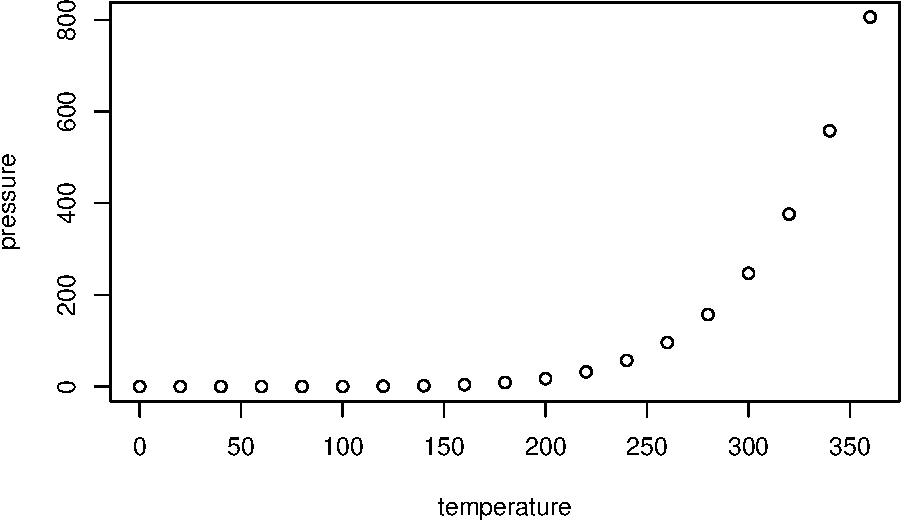
\includegraphics{thesis_files/figure-latex/pressure-1.pdf}

Note that the \texttt{echo=FALSE} parameter was added to the code chunk
to prevent printing of the \textbf{R} code that generated the plot.
There are plenty of other ways to add chunk options. More information is
available at \url{http://yihui.name/knitr/options/}.

Another useful chunk option is the setting of \texttt{cache=TRUE} as you
see here. If document rendering becomes time consuming due to long
computations or plots that are expensive to generate you can use knitr
caching to improve performance. Later in this file, you'll see a way to
reference plots created in \textbf{R} or external figures.

\hypertarget{loading-and-exploring-data}{%
\section{Loading and exploring data}\label{loading-and-exploring-data}}

Included in this template is a file called \texttt{flights.csv}. This
file includes a subset of the larger dataset of information about all
flights that departed from Seattle and Portland in 2014. More
information about this dataset and its \textbf{R} package is available
at \url{http://github.com/ismayc/pnwflights14}. This subset includes
only Portland flights and only rows that were complete with no missing
values. Merges were also done with the \texttt{airports} and
\texttt{airlines} data sets in the \texttt{pnwflights14} package to get
more descriptive airport and airline names.

We can load in this data set using the following command:
\begin{Shaded}
\begin{Highlighting}[]
\NormalTok{flights <-}\StringTok{ }\KeywordTok{read.csv}\NormalTok{(}\StringTok{"data/flights.csv"}\NormalTok{)}
\end{Highlighting}
\end{Shaded}
The data is now stored in the data frame called \texttt{flights} in
\textbf{R}. To get a better feel for the variables included in this
dataset we can use a variety of functions. Here we can see the
dimensions (rows by columns) and also the names of the columns.
\begin{Shaded}
\begin{Highlighting}[]
\KeywordTok{dim}\NormalTok{(flights)}
\end{Highlighting}
\end{Shaded}
\begin{verbatim}
[1] 52808    16
\end{verbatim}
\begin{Shaded}
\begin{Highlighting}[]
\KeywordTok{names}\NormalTok{(flights)}
\end{Highlighting}
\end{Shaded}
\begin{verbatim}
 [1] "month"        "day"          "dep_time"     "dep_delay"   
 [5] "arr_time"     "arr_delay"    "carrier"      "tailnum"     
 [9] "flight"       "dest"         "air_time"     "distance"    
[13] "hour"         "minute"       "carrier_name" "dest_name"   
\end{verbatim}
Another good idea is to take a look at the dataset in table form. With
this dataset having more than 50,000 rows, we won't explicitly show the
results of the command here. I recommend you enter the command into the
Console \textbf{\emph{after}} you have run the \textbf{R} chunks above
to load the data into \textbf{R}.
\begin{Shaded}
\begin{Highlighting}[]
\KeywordTok{View}\NormalTok{(flights)}
\end{Highlighting}
\end{Shaded}
While not required, it is highly recommended you use the \texttt{dplyr}
package to manipulate and summarize your data set as needed. It uses a
syntax that is easy to understand using chaining operations. Below I've
created a few examples of using \texttt{dplyr} to get information about
the Portland flights in 2014. You will also see the use of the
\texttt{ggplot2} package, which produces beautiful, high-quality
academic visuals.

We begin by checking to ensure that needed packages are installed and
then we load them into our current working environment:
\begin{Shaded}
\begin{Highlighting}[]
\CommentTok{# List of packages required for this analysis}
\NormalTok{pkg <-}\StringTok{ }\KeywordTok{c}\NormalTok{(}\StringTok{"dplyr"}\NormalTok{, }\StringTok{"ggplot2"}\NormalTok{, }\StringTok{"knitr"}\NormalTok{, }\StringTok{"bookdown"}\NormalTok{, }\StringTok{"devtools"}\NormalTok{)}
\CommentTok{# Check if packages are not installed and assign the}
\CommentTok{# names of the packages not installed to the variable new.pkg}
\NormalTok{new.pkg <-}\StringTok{ }\NormalTok{pkg[}\OperatorTok{!}\NormalTok{(pkg }\OperatorTok\StringTok{ }\KeywordTok{installed.packages}\NormalTok{())]}
\CommentTok{# If there are any packages in the list that aren't installed,}
\CommentTok{# install them}
\ControlFlowTok{if}\NormalTok{ (}\KeywordTok{length}\NormalTok{(new.pkg))}
  \KeywordTok{install.packages}\NormalTok{(new.pkg, }\DataTypeTok{repos =} \StringTok{"http://cran.rstudio.com"}\NormalTok{)}
\CommentTok{# Load packages (huskydown will load all of the packages as well)}
\KeywordTok{library}\NormalTok{(huskydown)}
\end{Highlighting}
\end{Shaded}
\clearpage

The example we show here does the following:
\begin{itemize}
\item
  Selects only the \texttt{carrier\_name} and \texttt{arr\_delay} from
  the \texttt{flights} dataset and then assigns this subset to a new
  variable called \texttt{flights2}.
\item
  Using \texttt{flights2}, we determine the largest arrival delay for
  each of the carriers.
\end{itemize}
\begin{Shaded}
\begin{Highlighting}[]
\KeywordTok{library}\NormalTok{(dplyr)}
\end{Highlighting}
\end{Shaded}
\begin{verbatim}

Attaching package: 'dplyr'
\end{verbatim}
\begin{verbatim}
The following objects are masked from 'package:stats':

    filter, lag
\end{verbatim}
\begin{verbatim}
The following object is masked from '.env':

    n
\end{verbatim}
\begin{verbatim}
The following objects are masked from 'package:base':

    intersect, setdiff, setequal, union
\end{verbatim}
\begin{Shaded}
\begin{Highlighting}[]
\NormalTok{flights2 <-}\StringTok{ }\NormalTok{flights }\OperatorTok\StringTok{ }
\StringTok{  }\KeywordTok{select}\NormalTok{(carrier_name, arr_delay)}
\NormalTok{max_delays <-}\StringTok{ }\NormalTok{flights2 }\OperatorTok\StringTok{ }
\StringTok{  }\KeywordTok{group_by}\NormalTok{(carrier_name) }\OperatorTok
\StringTok{  }\KeywordTok{summarize}\NormalTok{(}\DataTypeTok{max_arr_delay =} \KeywordTok{max}\NormalTok{(arr_delay, }\DataTypeTok{na.rm =} \OtherTok{TRUE}\NormalTok{))}
\end{Highlighting}
\end{Shaded}
A useful function in the \texttt{knitr} package for making nice tables
in \emph{R Markdown} is called \texttt{kable}. It is much easier to use
than manually entering values into a table by copying and pasting values
into Excel or LaTeX. This again goes to show how nice reproducible
documents can be! (Note the use of \texttt{results="asis"}, which will
produce the table instead of the code to create the table.) The
\texttt{caption.short} argument is used to include a shorter title to
appear in the List of Tables.
\begin{Shaded}
\begin{Highlighting}[]
\KeywordTok{library}\NormalTok{(knitr)}
\KeywordTok{kable}\NormalTok{(max_delays, }
      \DataTypeTok{col.names =} \KeywordTok{c}\NormalTok{(}\StringTok{"Airline"}\NormalTok{, }\StringTok{"Max Arrival Delay"}\NormalTok{),}
      \DataTypeTok{caption =} \StringTok{"Maximum Delays by Airline"}\NormalTok{,}
      \DataTypeTok{caption.short =} \StringTok{"Max Delays by Airline"}\NormalTok{,}
      \DataTypeTok{longtable =} \OtherTok{TRUE}\NormalTok{,}
      \DataTypeTok{booktabs =} \OtherTok{TRUE}\NormalTok{)}
\end{Highlighting}
\end{Shaded}
\begin{longtable}[t]{lr}
\caption[Max Delays by Airline]{\label{tab:maxdelays}Maximum Delays by Airline}\\
\toprule
Airline & Max Arrival Delay\\
\midrule
Alaska Airlines Inc. & 338\\
American Airlines Inc. & 1539\\
Delta Air Lines Inc. & 651\\
Frontier Airlines Inc. & 575\\
Hawaiian Airlines Inc. & 407\\
\addlinespace
JetBlue Airways & 273\\
SkyWest Airlines Inc. & 421\\
Southwest Airlines Co. & 694\\
United Air Lines Inc. & 472\\
US Airways Inc. & 347\\
Virgin America & 366\\
\bottomrule
\end{longtable}
The last two options make the table a little easier-to-read.

We can further look into the properties of the largest value here for
American Airlines Inc.~To do so, we can isolate the row corresponding to
the arrival delay of 1539 minutes for American in our original
\texttt{flights} dataset.
\begin{Shaded}
\begin{Highlighting}[]
\NormalTok{flights }\OperatorTok\StringTok{ }
\StringTok{  }\KeywordTok{filter}\NormalTok{(arr_delay }\OperatorTok{==}\StringTok{ }\DecValTok{1539}\NormalTok{, }
\NormalTok{         carrier_name }\OperatorTok{==}\StringTok{ "American Airlines Inc."}\NormalTok{) }\OperatorTok
\StringTok{  }\KeywordTok{select}\NormalTok{(}\OperatorTok{-}\KeywordTok{c}\NormalTok{(month, day, carrier, dest_name, hour, }
\NormalTok{            minute, carrier_name, arr_delay))}
\end{Highlighting}
\end{Shaded}
\begin{verbatim}
  dep_time dep_delay arr_time tailnum flight dest air_time distance
1     1403      1553     1934  N595AA   1568  DFW      182     1616
\end{verbatim}
We see that the flight occurred on March 3rd and departed a little after
2 PM on its way to Dallas/Fort Worth. Lastly, we show how we can
visualize the arrival delay of all departing flights from Portland on
March 3rd against time of departure.
\begin{Shaded}
\begin{Highlighting}[]
\KeywordTok{library}\NormalTok{(ggplot2)}
\NormalTok{flights }\OperatorTok\StringTok{ }
\StringTok{  }\KeywordTok{filter}\NormalTok{(month }\OperatorTok{==}\StringTok{ }\DecValTok{3}\NormalTok{, day }\OperatorTok{==}\StringTok{ }\DecValTok{3}\NormalTok{) }\OperatorTok
\StringTok{  }\KeywordTok{ggplot}\NormalTok{(}\KeywordTok{aes}\NormalTok{(}\DataTypeTok{x =}\NormalTok{ dep_time, }
             \DataTypeTok{y =}\NormalTok{ arr_delay)) }\OperatorTok{+}\StringTok{ }
\StringTok{  }\KeywordTok{geom_point}\NormalTok{()}
\end{Highlighting}
\end{Shaded}
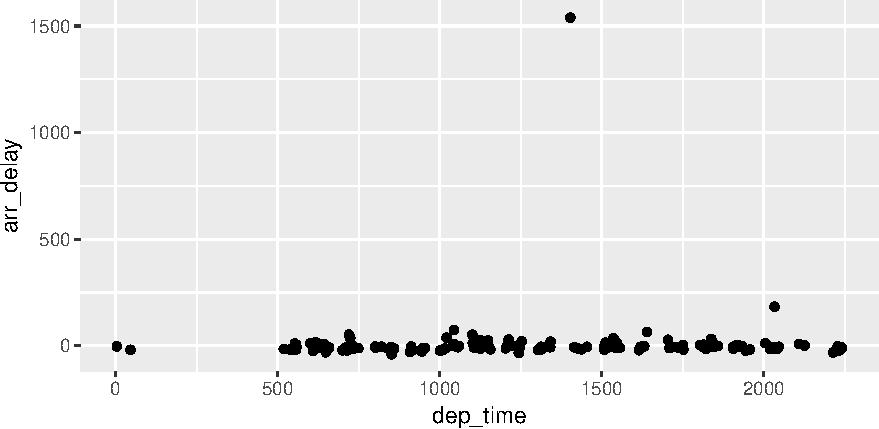
\includegraphics{thesis_files/figure-latex/march3plot-1.pdf}

\hypertarget{additional-resources}{%
\section{Additional resources}\label{additional-resources}}
\begin{itemize}
\item
  \emph{Markdown} Cheatsheet -
  \url{https://github.com/adam-p/markdown-here/wiki/Markdown-Cheatsheet}
\item
  \emph{R Markdown} Reference Guide -
  \url{https://www.rstudio.com/wp-content/uploads/2015/03/rmarkdown-reference.pdf}
\item
  Introduction to \texttt{dplyr} -
  \url{https://cran.rstudio.com/web/packages/dplyr/vignettes/introduction.html}
\item
  \texttt{ggplot2} Documentation -
  \url{http://docs.ggplot2.org/current/}
\end{itemize}
\hypertarget{math-sci}{%
\chapter{Mathematics and Science}\label{math-sci}}

\hypertarget{math}{%
\section{Math}\label{math}}

\TeX~is the best way to typeset mathematics. Donald Knuth designed
\TeX~when he got frustrated at how long it was taking the typesetters to
finish his book, which contained a lot of mathematics. One nice feature
of \emph{R Markdown} is its ability to read LaTeX code directly.

If you are doing a thesis that will involve lots of math, you will want
to read the following section which has been commented out. If you're
not going to use math, skip over or delete this next commented section.

\hypertarget{chemistry-101-symbols}{%
\section{Chemistry 101: Symbols}\label{chemistry-101-symbols}}

Chemical formulas will look best if they are not italicized. Get around
math mode's automatic italicizing in LaTeX by using the argument
\texttt{\$\textbackslash{}mathrm\{formula\ here\}\$}, with your formula
inside the curly brackets. (Notice the use of the backticks here which
enclose text that acts as code.)

So, \(\mathrm{Fe_2^{2+}Cr_2O_4}\) is written
\texttt{\$\textbackslash{}mathrm\{Fe\_2\^{}\{2+\}Cr\_2O\_4\}\$}.

\noindent Exponent or Superscript: \(\mathrm{O^-}\)

\noindent Subscript: \(\mathrm{CH_4}\)

To stack numbers or letters as in \(\mathrm{Fe_2^{2+}}\), the subscript
is defined first, and then the superscript is defined.

\noindent Bullet: CuCl \(\bullet\) \(\mathrm{7H_{2}O}\)

\noindent Delta: \(\Delta\)

\noindent Reaction Arrows: \(\longrightarrow\) or
\(\xrightarrow{solution}\)

\noindent Resonance Arrows: \(\leftrightarrow\)

\noindent Reversible Reaction Arrows: \(\rightleftharpoons\)

\hypertarget{typesetting-reactions}{%
\subsection{Typesetting reactions}\label{typesetting-reactions}}

You may wish to put your reaction in an equation environment, which
means that LaTeX will place the reaction where it fits and will number
the equations for you.
\begin{equation}
  \mathrm{C_6H_{12}O_6  + 6O_2} \longrightarrow \mathrm{6CO_2 + 6H_2O}
  \label{eq:reaction}
\end{equation}
We can reference this combustion of glucose reaction via Equation
\eqref{eq:reaction}.

\hypertarget{other-examples-of-reactions}{%
\subsection{Other examples of
reactions}\label{other-examples-of-reactions}}

\(\mathrm{NH_4Cl_{(s)}}\) \(\rightleftharpoons\)
\(\mathrm{NH_{3(g)}+HCl_{(g)}}\)

\noindent \(\mathrm{MeCH_2Br + Mg}\) \(\xrightarrow[below]{above}\)
\(\mathrm{MeCH_2\bullet Mg \bullet Br}\)

\hypertarget{physics}{%
\section{Physics}\label{physics}}

Many of the symbols you will need can be found on the math page
\url{http://web.reed.edu/cis/help/latex/math.html} and the Comprehensive
LaTeX Symbol Guide
(\url{http://mirror.utexas.edu/ctan/info/symbols/comprehensive/symbols-letter.pdf}).

\hypertarget{biology}{%
\section{Biology}\label{biology}}

You will probably find the resources at
\url{http://www.lecb.ncifcrf.gov/~toms/latex.html} helpful, particularly
the links to bsts for various journals. You may also be interested in
TeXShade for nucleotide typesetting
(\url{http://homepages.uni-tuebingen.de/beitz/txe.html}). Be sure to
read the proceeding chapter on graphics and tables.

\hypertarget{ref-labels}{%
\chapter{Tables, Graphics, References, and Labels}\label{ref-labels}}

\hypertarget{tables}{%
\section{Tables}\label{tables}}

By far the easiest way to present tables in your thesis is to store the
contents of the table in a CSV or Excel file, then read that file in to
your R Markdown document as a data frame. Then you can style the table
with the \texttt{kable} function, or functions in the
\href{https://cran.r-project.org/web/packages/kableExtra/index.html}{kableExtra}
pacakge.

In addition to the tables that can be automatically generated from a
data frame in \textbf{R} that you saw in
\protect\hyperlink{rmd-basics}{R Markdown Basics} using the
\texttt{kable} function, you can also create tables using \emph{pandoc}.
(More information is available at
\url{http://pandoc.org/README.html\#tables}.) This might be useful if
you don't have values specifically stored in \textbf{R}, but you'd like
to display them in table form. Below is an example. Pay careful
attention to the alignment in the table and hyphens to create the rows
and columns. Generally I don't recommend this approach of typing the
table directly into your R Markdown document.
\begin{longtable}[]{@{}ccc@{}}
\caption{\label{tab:inher} Correlation of Inheritance Factors for Parents
and Child}\tabularnewline
\toprule
\begin{minipage}[b]{0.29\columnwidth}\centering
Factors\strut
\end{minipage} & \begin{minipage}[b]{0.46\columnwidth}\centering
Correlation between Parents \& Child\strut
\end{minipage} & \begin{minipage}[b]{0.16\columnwidth}\centering
Inherited\strut
\end{minipage}\tabularnewline
\midrule
\endfirsthead
\toprule
\begin{minipage}[b]{0.29\columnwidth}\centering
Factors\strut
\end{minipage} & \begin{minipage}[b]{0.46\columnwidth}\centering
Correlation between Parents \& Child\strut
\end{minipage} & \begin{minipage}[b]{0.16\columnwidth}\centering
Inherited\strut
\end{minipage}\tabularnewline
\midrule
\endhead
\begin{minipage}[t]{0.29\columnwidth}\centering
Education\strut
\end{minipage} & \begin{minipage}[t]{0.46\columnwidth}\centering
-0.49\strut
\end{minipage} & \begin{minipage}[t]{0.16\columnwidth}\centering
Yes\strut
\end{minipage}\tabularnewline
\begin{minipage}[t]{0.29\columnwidth}\centering
Socio-Economic Status\strut
\end{minipage} & \begin{minipage}[t]{0.46\columnwidth}\centering
0.28\strut
\end{minipage} & \begin{minipage}[t]{0.16\columnwidth}\centering
Slight\strut
\end{minipage}\tabularnewline
\begin{minipage}[t]{0.29\columnwidth}\centering
Income\strut
\end{minipage} & \begin{minipage}[t]{0.46\columnwidth}\centering
0.08\strut
\end{minipage} & \begin{minipage}[t]{0.16\columnwidth}\centering
No\strut
\end{minipage}\tabularnewline
\begin{minipage}[t]{0.29\columnwidth}\centering
Family Size\strut
\end{minipage} & \begin{minipage}[t]{0.46\columnwidth}\centering
0.18\strut
\end{minipage} & \begin{minipage}[t]{0.16\columnwidth}\centering
Slight\strut
\end{minipage}\tabularnewline
\begin{minipage}[t]{0.29\columnwidth}\centering
Occupational Prestige\strut
\end{minipage} & \begin{minipage}[t]{0.46\columnwidth}\centering
0.21\strut
\end{minipage} & \begin{minipage}[t]{0.16\columnwidth}\centering
Slight\strut
\end{minipage}\tabularnewline
\bottomrule
\end{longtable}
We can also create a link to the table by doing the following: Table
\ref{tab:inher}. If you go back to
\protect\hyperlink{loading-and-exploring-data}{Loading and exploring
data} and look at the \texttt{kable} table, we can create a reference to
this max delays table too: Table \ref{tab:maxdelays}. The addition of
the \texttt{(\textbackslash{}\#tab:inher)} option to the end of the
table caption allows us to then make a reference to Table
\texttt{\textbackslash{}@ref(tab:label)}. Note that this reference could
appear anywhere throughout the document after the table has appeared.

\clearpage

\hypertarget{figures}{%
\section{Figures}\label{figures}}

If your thesis has a lot of figures, \emph{R Markdown} might behave
better for you than that other word processor. One perk is that it will
automatically number the figures accordingly in each chapter. You'll
also be able to create a label for each figure, add a caption, and then
reference the figure in a way similar to what we saw with tables
earlier. If you label your figures, you can move the figures around and
\emph{R Markdown} will automatically adjust the numbering for you. No
need for you to remember! So that you don't have to get too far into
LaTeX to do this, a couple \textbf{R} functions have been created for
you to assist. You'll see their use below.

In the \textbf{R} chunk below, we will load in a picture stored as
\texttt{uw.png} in our main directory. We then give it the caption of
``UW logo'', the label of ``uwlogo'', and specify that this is a figure.
Make note of the different \textbf{R} chunk options that are given in
the R Markdown file (not shown in the knitted document).
\begin{Shaded}
\begin{Highlighting}[]
\KeywordTok{include_graphics}\NormalTok{(}\DataTypeTok{path =} \StringTok{"figure/uw.png"}\NormalTok{)}
\end{Highlighting}
\end{Shaded}
\begin{figure}

\includegraphics[width=6.25in]{figure/uw} \caption{UW logo}\label{fig:uwlogo}
\end{figure}
Here is a reference to the UW logo: Figure \ref{fig:uwlogo}. Note the
use of the \texttt{fig:} code here. By naming the \textbf{R} chunk that
contains the figure, we can then reference that figure later as done in
the first sentence here. We can also specify the caption for the figure
via the R chunk option \texttt{fig.cap}.

\clearpage

Below we will investigate how to save the output of an \textbf{R} plot
and label it in a way similar to that done above. Recall the
\texttt{flights} dataset from Chapter \ref{rmd-basics}. (Note that we've
shown a different way to reference a section or chapter here.) We will
next explore a bar graph with the mean flight departure delays by
airline from Portland for 2014. Note also the use of the \texttt{scale}
parameter which is discussed on the next page.
\begin{Shaded}
\begin{Highlighting}[]
\NormalTok{flights }\OperatorTok\StringTok{ }\KeywordTok{group_by}\NormalTok{(carrier) }\OperatorTok
\StringTok{  }\KeywordTok{summarize}\NormalTok{(}\DataTypeTok{mean_dep_delay =} \KeywordTok{mean}\NormalTok{(dep_delay)) }\OperatorTok
\StringTok{  }\KeywordTok{ggplot}\NormalTok{(}\KeywordTok{aes}\NormalTok{(}\DataTypeTok{x =}\NormalTok{ carrier, }\DataTypeTok{y =}\NormalTok{ mean_dep_delay)) }\OperatorTok{+}
\StringTok{  }\KeywordTok{geom_bar}\NormalTok{(}\DataTypeTok{position =} \StringTok{"identity"}\NormalTok{, }\DataTypeTok{stat =} \StringTok{"identity"}\NormalTok{, }\DataTypeTok{fill =} \StringTok{"red"}\NormalTok{)}
\end{Highlighting}
\end{Shaded}
\begin{figure}
\centering
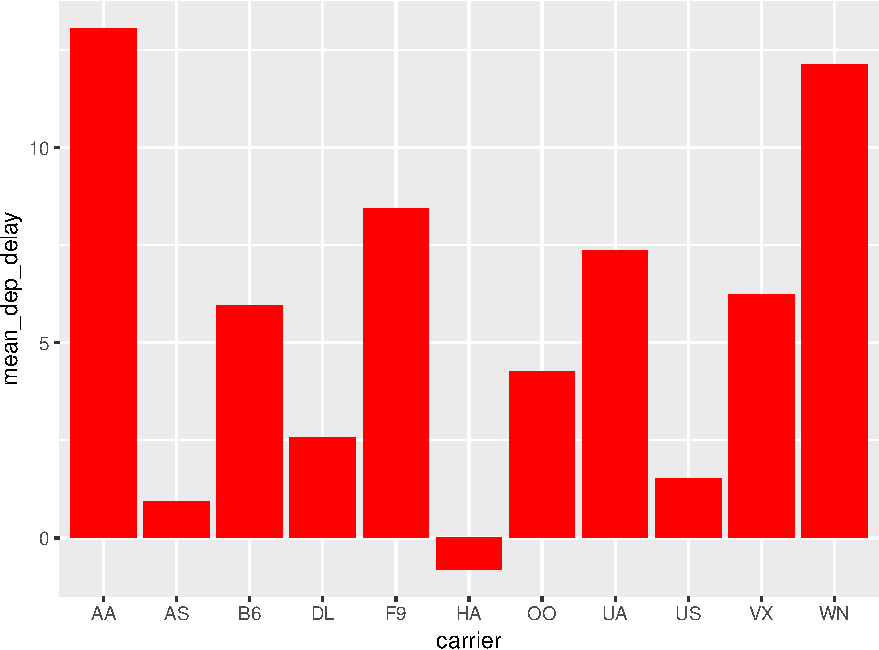
\includegraphics{thesis_files/figure-latex/delaysboxplot-1.pdf}
\caption{\label{fig:delaysboxplot}Mean Delays by Airline}
\end{figure}
Here is a reference to this image: Figure \ref{fig:delaysboxplot}.

A table linking these carrier codes to airline names is available at
\url{https://github.com/ismayc/pnwflights14/blob/master/data/airlines.csv}.

\clearpage

Next, we will explore the use of the \texttt{out.extra} chunk option,
which can be used to shrink or expand an image loaded from a file by
specifying \texttt{"scale=\ "}. Here we use the mathematical graph
stored in the ``subdivision.pdf'' file.
\begin{figure}
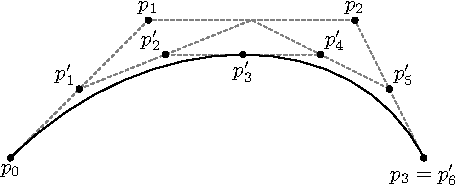
\includegraphics[scale=0.75]{figure/subdivision} \caption{Subdiv. graph}\label{fig:subd}
\end{figure}
Here is a reference to this image: Figure \ref{fig:subd}. Note that
\texttt{echo=FALSE} is specified so that the \textbf{R} code is hidden
in the document.

\textbf{More Figure Stuff}

Lastly, we will explore how to rotate and enlarge figures using the
\texttt{out.extra} chunk option. (Currently this only works in the PDF
version of the book.)
\begin{figure}
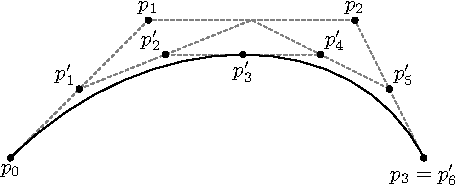
\includegraphics[angle=180, scale=1.1]{figure/subdivision} \caption{A Larger Figure, Flipped Upside Down}\label{fig:subd2}
\end{figure}
As another example, here is a reference: Figure \ref{fig:subd2}.

\hypertarget{footnotes-and-endnotes}{%
\section{Footnotes and Endnotes}\label{footnotes-and-endnotes}}

You might want to footnote something.\footnote{footnote text} The
footnote will be in a smaller font and placed appropriately. Endnotes
work in much the same way.

\hypertarget{bibliographies}{%
\section{Bibliographies}\label{bibliographies}}

Of course you will need to cite things, and you will probably accumulate
an armful of sources. There are a variety of tools available for
creating a bibliography database (stored with the .bib extension). In
addition to BibTeX suggested below, you may want to consider using the
free and easy-to-use tool called Zotero. Some Zotero documentation is at
\url{http://libguides.reed.edu/citation/zotero}. In addition, a tutorial
is available from Middlebury College at
\url{http://sites.middlebury.edu/zoteromiddlebury/}.

\emph{R Markdown} uses \emph{pandoc} (\url{http://pandoc.org/}) to build
its bibliographies. One nice caveat of this is that you won't have to do
a second compile to load in references as standard LaTeX requires. To
cite references in your thesis (after creating your bibliography
database), place the reference name inside square brackets and precede
it by the ``at'' symbol. For example, here's a reference to a book about
worrying: (Molina \& Borkovec, 1994). This \texttt{Molina1994} entry
appears in a file called \texttt{thesis.bib} in the \texttt{bib} folder.
This bibliography database file was created by a program called BibTeX.
You can call this file something else if you like (look at the YAML
header in the main .Rmd file) and, by default, is to placed in the
\texttt{bib} folder.

For more information about BibTeX and bibliographies, see
(\url{http://web.reed.edu/cis/help/latex/index.html})\footnote{Reed~College
  (2007)}. There are three pages on this topic: \emph{bibtex} (which
talks about using BibTeX, at
\url{http://web.reed.edu/cis/help/latex/bibtex.html}),
\emph{bibtexstyles} (about how to find and use the bibliography style
that best suits your needs, at
\url{http://web.reed.edu/cis/help/latex/bibtexstyles.html}) and
\emph{bibman} (which covers how to make and maintain a bibliography by
hand, without BibTeX, at
\url{http://web.reed.edu/cis/help/latex/bibman.html}). The last page
will not be useful unless you have only a few sources.

If you look at the YAML header at the top of the main .Rmd file you can
see that we can specify the style of the bibliography by referencing the
appropriate csl file. You can download a variety of different style
files at \url{https://www.zotero.org/styles}. Make sure to download the
file into the csl folder.

\textbf{Tips for Bibliographies}
\begin{itemize}
\tightlist
\item
  Like with thesis formatting, the sooner you start compiling your
  bibliography for something as large as thesis, the better.
\item
  The cite key (a citation's label) needs to be unique from the other
  entries.
\item
  When you have more than one author or editor, you need to separate
  each author's name by the word ``and'' e.g.
  \texttt{Author\ =\ \{Noble,\ Sam\ and\ Youngberg,\ Jessica\},}.
\item
  Bibliographies made using BibTeX (whether manually or using a manager)
  accept LaTeX markup, so you can italicize and add symbols as
  necessary.
\item
  To force capitalization in an article title or where all lowercase is
  generally used, bracket the capital letter in curly braces.
\end{itemize}
\hypertarget{anything-else}{%
\section{Anything else?}\label{anything-else}}

If you'd like to see examples of other things in this template, please
\href{https://github.com/benmarwick/huskydown/issues/new}{contact us}
(email \href{mailto:bmarwick@uw.edu}{\nolinkurl{bmarwick@uw.edu}}) with
your suggestions. We love to see people using \emph{R Markdown} for
their theses, and are happy to help.

\hypertarget{conclusion}{%
\chapter*{Conclusion}\label{conclusion}}
\addcontentsline{toc}{chapter}{Conclusion}

If we don't want Conclusion to have a chapter number next to it, we can
add the \texttt{\{-\}} attribute.

\textbf{More info}

And here's some other random info: the first paragraph after a chapter
title or section head \emph{shouldn't be} indented, because indents are
to tell the reader that you're starting a new paragraph. Since that's
obvious after a chapter or section title, proper typesetting doesn't add
an indent there.

\appendix

\hypertarget{the-first-appendix}{%
\chapter{The First Appendix}\label{the-first-appendix}}

This first appendix includes all of the R chunks of code that were
hidden throughout the document (using the \texttt{include\ =\ FALSE}
chunk tag) to help with readibility and/or setup.

\textbf{In the main Rmd file}
\begin{Shaded}
\begin{Highlighting}[]
\CommentTok{# This chunk ensures that the huskydown package is}
\CommentTok{# installed and loaded. This huskydown package includes}
\CommentTok{# the template files for the thesis.}
\ControlFlowTok{if}\NormalTok{(}\OperatorTok{!}\KeywordTok{require}\NormalTok{(devtools))}
  \KeywordTok{install.packages}\NormalTok{(}\StringTok{"devtools"}\NormalTok{, }\DataTypeTok{repos =} \StringTok{"http://cran.rstudio.com"}\NormalTok{)}
\ControlFlowTok{if}\NormalTok{(}\OperatorTok{!}\KeywordTok{require}\NormalTok{(huskydown))}
\NormalTok{  devtools}\OperatorTok{::}\KeywordTok{install_github}\NormalTok{(}\StringTok{"benmarwick/huskydown"}\NormalTok{)}
\KeywordTok{library}\NormalTok{(huskydown)}
\CommentTok{#if(!require(huskydown))}
\CommentTok{#  devtools::install_github("danovando/gauchodown")}
\CommentTok{#library(gauchodown)}
\end{Highlighting}
\end{Shaded}
\textbf{In Chapter \ref{ref-labels}:}
\begin{Shaded}
\begin{Highlighting}[]
\CommentTok{# This chunk ensures that the huskydown package is}
\CommentTok{# installed and loaded. This huskydown package includes}
\CommentTok{# the template files for the thesis and also two functions}
\CommentTok{# used for labeling and referencing}
\ControlFlowTok{if}\NormalTok{(}\OperatorTok{!}\KeywordTok{require}\NormalTok{(devtools))}
  \KeywordTok{install.packages}\NormalTok{(}\StringTok{"devtools"}\NormalTok{, }\DataTypeTok{repos =} \StringTok{"http://cran.rstudio.com"}\NormalTok{)}
\ControlFlowTok{if}\NormalTok{(}\OperatorTok{!}\KeywordTok{require}\NormalTok{(dplyr))}
    \KeywordTok{install.packages}\NormalTok{(}\StringTok{"dplyr"}\NormalTok{, }\DataTypeTok{repos =} \StringTok{"http://cran.rstudio.com"}\NormalTok{)}
\ControlFlowTok{if}\NormalTok{(}\OperatorTok{!}\KeywordTok{require}\NormalTok{(ggplot2))}
    \KeywordTok{install.packages}\NormalTok{(}\StringTok{"ggplot2"}\NormalTok{, }\DataTypeTok{repos =} \StringTok{"http://cran.rstudio.com"}\NormalTok{)}
\ControlFlowTok{if}\NormalTok{(}\OperatorTok{!}\KeywordTok{require}\NormalTok{(ggplot2))}
    \KeywordTok{install.packages}\NormalTok{(}\StringTok{"bookdown"}\NormalTok{, }\DataTypeTok{repos =} \StringTok{"http://cran.rstudio.com"}\NormalTok{)}
\ControlFlowTok{if}\NormalTok{(}\OperatorTok{!}\KeywordTok{require}\NormalTok{(huskydown))\{}
  \KeywordTok{library}\NormalTok{(devtools)}
\NormalTok{  devtools}\OperatorTok{::}\KeywordTok{install_github}\NormalTok{(}\StringTok{"benmarwick/huskydown"}\NormalTok{)}
\NormalTok{  \}}
\KeywordTok{library}\NormalTok{(huskydown)}
\NormalTok{flights <-}\StringTok{ }\KeywordTok{read.csv}\NormalTok{(}\StringTok{"data/flights.csv"}\NormalTok{)}
\end{Highlighting}
\end{Shaded}
\hypertarget{the-second-appendix-for-fun}{%
\chapter{The Second Appendix, for
Fun}\label{the-second-appendix-for-fun}}

\hypertarget{colophon}{%
\chapter*{Colophon}\label{colophon}}
\addcontentsline{toc}{chapter}{Colophon}

This document is set in \href{https://github.com/georgd/EB-Garamond}{EB
Garamond}, \href{https://github.com/adobe-fonts/source-code-pro/}{Source
Code Pro} and \href{http://www.latofonts.com/lato-free-fonts/}{Lato}.
The body text is set at 11pt with \(\familydefault\).

It was written in R Markdown and \(\LaTeX\), and rendered into PDF using
\href{https://github.com/benmarwick/huskydown}{huskydown} and
\href{https://github.com/rstudio/bookdown}{bookdown}.

This document was typeset using the XeTeX typesetting system, and the
\href{http://staff.washington.edu/fox/tex/}{University of Washington
Thesis class} class created by Jim Fox. Under the hood, the
\href{https://github.com/UWIT-IAM/UWThesis}{University of Washington
Thesis LaTeX template} is used to ensure that documents conform
precisely to submission standards. Other elements of the document
formatting source code have been taken from the
\href{https://github.com/stevenpollack/ucbthesis}{Latex, Knitr, and
RMarkdown templates for UC Berkeley's graduate thesis}, and
\href{https://github.com/suchow/Dissertate}{Dissertate: a LaTeX
dissertation template to support the production and typesetting of a PhD
dissertation at Harvard, Princeton, and NYU}

The source files for this thesis, along with all the data files, have
been organised into an R package, xxx, which is available at
\url{https://github.com/xxx/xxx}. A hard copy of the thesis can be found
in the University of Washington library.

This version of the thesis was generated on 2018-07-30 17:13:39. The
repository is currently at this commit:

The computational environment that was used to generate this version is
as follows:
\begin{verbatim}
Session info -------------------------------------------------------------
\end{verbatim}
\begin{verbatim}
 setting  value                       
 version  R version 3.5.1 (2018-07-02)
 system   x86_64, darwin15.6.0        
 ui       X11                         
 language (EN)                        
 collate  en_US.UTF-8                 
 tz       America/Los_Angeles         
 date     2018-07-30                  
\end{verbatim}
\begin{verbatim}
Packages -----------------------------------------------------------------
\end{verbatim}
\begin{verbatim}
 package    * version    date       source                               
 assertthat   0.2.0      2017-04-11 CRAN (R 3.5.0)                       
 backports    1.1.2      2017-12-13 CRAN (R 3.5.0)                       
 base       * 3.5.1      2018-07-05 local                                
 bindr        0.1.1      2018-03-13 CRAN (R 3.5.0)                       
 bindrcpp   * 0.2.2      2018-03-29 CRAN (R 3.5.0)                       
 bookdown     0.7.15     2018-07-30 Github (rstudio/bookdown@c470a52)    
 codetools    0.2-15     2016-10-05 CRAN (R 3.5.1)                       
 colorspace   1.3-2      2016-12-14 CRAN (R 3.5.0)                       
 compiler     3.5.1      2018-07-05 local                                
 crayon       1.3.4      2017-09-16 CRAN (R 3.5.0)                       
 datasets   * 3.5.1      2018-07-05 local                                
 devtools   * 1.13.6     2018-06-27 CRAN (R 3.5.0)                       
 digest       0.6.15     2018-01-28 CRAN (R 3.5.0)                       
 dplyr      * 0.7.6      2018-06-29 CRAN (R 3.5.0)                       
 evaluate     0.11       2018-07-17 CRAN (R 3.5.0)                       
 ggplot2    * 3.0.0.9000 2018-07-30 Github (tidyverse/ggplot2@1021646)   
 git2r        0.23.0     2018-07-17 CRAN (R 3.5.0)                       
 glue         1.3.0      2018-07-17 CRAN (R 3.5.0)                       
 graphics   * 3.5.1      2018-07-05 local                                
 grDevices  * 3.5.1      2018-07-05 local                                
 grid         3.5.1      2018-07-05 local                                
 gtable       0.2.0      2016-02-26 CRAN (R 3.5.0)                       
 highr        0.7        2018-06-09 CRAN (R 3.5.0)                       
 htmltools    0.3.6      2017-04-28 CRAN (R 3.5.0)                       
 huskydown  * 0.0.5      2018-07-30 Github (danovando/gauchodown@5a18965)
 knitr      * 1.20       2018-02-20 CRAN (R 3.5.0)                       
 labeling     0.3        2014-08-23 CRAN (R 3.5.0)                       
 lazyeval     0.2.1      2017-10-29 CRAN (R 3.5.0)                       
 magrittr     1.5        2014-11-22 CRAN (R 3.5.0)                       
 memoise      1.1.0      2017-04-21 CRAN (R 3.5.0)                       
 methods    * 3.5.1      2018-07-05 local                                
 munsell      0.5.0      2018-06-12 CRAN (R 3.5.0)                       
 pillar       1.3.0      2018-07-14 CRAN (R 3.5.0)                       
 pkgconfig    2.0.1      2017-03-21 CRAN (R 3.5.0)                       
 plyr         1.8.4      2016-06-08 CRAN (R 3.5.0)                       
 png          0.1-7      2013-12-03 CRAN (R 3.5.0)                       
 purrr        0.2.5      2018-05-29 CRAN (R 3.5.0)                       
 R6           2.2.2      2017-06-17 CRAN (R 3.5.0)                       
 Rcpp         0.12.18    2018-07-23 CRAN (R 3.5.1)                       
 rlang        0.2.1      2018-05-30 CRAN (R 3.5.0)                       
 rmarkdown    1.10       2018-06-11 cran (@1.10)                         
 rprojroot    1.3-2      2018-01-03 CRAN (R 3.5.0)                       
 rstudioapi   0.7        2017-09-07 CRAN (R 3.5.0)                       
 scales       1.0.0      2018-07-30 Github (hadley/scales@9b82318)       
 stats      * 3.5.1      2018-07-05 local                                
 stringi      1.2.4      2018-07-20 CRAN (R 3.5.0)                       
 stringr      1.3.1      2018-05-10 CRAN (R 3.5.0)                       
 tibble       1.4.2      2018-01-22 CRAN (R 3.5.0)                       
 tidyselect   0.2.4      2018-02-26 CRAN (R 3.5.0)                       
 tools        3.5.1      2018-07-05 local                                
 utils      * 3.5.1      2018-07-05 local                                
 withr        2.1.2      2018-07-08 Github (jimhester/withr@fe56f20)     
 xfun         0.3        2018-07-06 CRAN (R 3.5.0)                       
 yaml         2.2.0      2018-07-25 CRAN (R 3.5.0)                       
\end{verbatim}
\backmatter

\hypertarget{references}{%
\chapter*{References}\label{references}}
\addcontentsline{toc}{chapter}{References}

\markboth{References}{References}

\noindent

\setlength{\parindent}{-0.20in}
\setlength{\leftskip}{0.20in}
\setlength{\parskip}{8pt}

\hypertarget{refs}{}
\leavevmode\hypertarget{ref-angel2000}{}%
Angel, E. (2000). \emph{Interactive computer graphics : A top-down
approach with opengl}. Boston, MA: Addison Wesley Longman.

\leavevmode\hypertarget{ref-angel2001}{}%
Angel, E. (2001a). \emph{Batch-file computer graphics : A bottom-up
approach with quicktime}. Boston, MA: Wesley Addison Longman.

\leavevmode\hypertarget{ref-angel2002a}{}%
Angel, E. (2001b). \emph{Test second book by angel}. Boston, MA: Wesley
Addison Longman.

\leavevmode\hypertarget{ref-Molina1994}{}%
Molina, S. T., \& Borkovec, T. D. (1994). The Penn State worry
questionnaire: Psychometric properties and associated characteristics.
In G. C. L. Davey \& F. Tallis (Eds.), \emph{Worrying: Perspectives on
theory, assessment and treatment} (pp. 265--283). New York: Wiley.

\leavevmode\hypertarget{ref-reedweb2007}{}%
Reed~College. (2007). LaTeX your document. Retrieved from
\url{http://web.reed.edu/cis/help/LaTeX/index.html}

\end{ucmainmatter}
\end{document}

%---Set Headers and Footers ------------------------------------------------------
\pagestyle{fancy}
\renewcommand{\chaptermark}[1]{\markboth{{\sf #1 \hspace*{\fill} Chapter~\thechapter}}{} }
\renewcommand{\sectionmark}[1]{\markright{ {\sf Section~\thesection \hspace*{\fill} #1 }}}
\fancyhf{}

\makeatletter \if@twoside \fancyhead[LO]{\small \rightmark} \fancyhead[RE]{\small\leftmark} \else \fancyhead[LO]{\small\leftmark}
\fancyhead[RE]{\small\rightmark} \fi

\def\cleardoublepage{\clearpage\if@openright \ifodd\c@page\else
  \hbox{}
  \vspace*{\fill}
  \begin{center}
    This page intentionally left blank
  \end{center}
  \vspace{\fill}
  \thispagestyle{plain}
  \newpage
  \fi \fi}
\makeatother
\fancyfoot[c]{\textrm{\textup{\thepage}}} % page number
\fancyfoot[C]{\thepage}
\renewcommand{\headrulewidth}{0.4pt}

\fancypagestyle{plain} { \fancyhf{} \fancyfoot[C]{\thepage}
\renewcommand{\headrulewidth}{0pt}
\renewcommand{\footrulewidth}{0pt}}
